\documentclass{beamer}
%Information to be included in the title page:
% \title{Sample title}
% \author{Anonymous}
% \institute{Overleaf}
\usepackage{booktabs}
\usepackage{graphicx}
\usepackage{subcaption}
\usepackage[]{hyperref}

\usetheme[]{default}
\begin{document}
\renewcommand{\d}{\: \mathrm{d} }
\newcommand{\e}{\mathrm{e}}


\title[] {Recitation Class for Mid I \\ Chapter 1-4}

\author[lzx]{Zexi Li}

\institute[email]{lzx12138@sjtu.edu.cn}

\date{2021.06.08}

\frame{\titlepage}

\AtBeginSection[]
{
  \begin{frame}
    \frametitle{Table of Contents}
    \tableofcontents[currentsection]
  \end{frame}
}

\begin{frame}
    \frametitle{Outline}
    \tableofcontents
\end{frame}


\section{Overview}
    \begin{frame} \frametitle{Overview}
        \begin{itemize}
            \item \textbf{Chapter 5} Carrier Transport Phenomena
                \begin{equation*}
                    J = qn\mu_n E_x+ qp\mu_p E_x + qD_n \nabla n + q D_p \nabla
                \end{equation*}
            \item \textbf{Chapter 4} The Semiconductor in Equilibrium
                \begin{figure}[H]
                    \centering
                    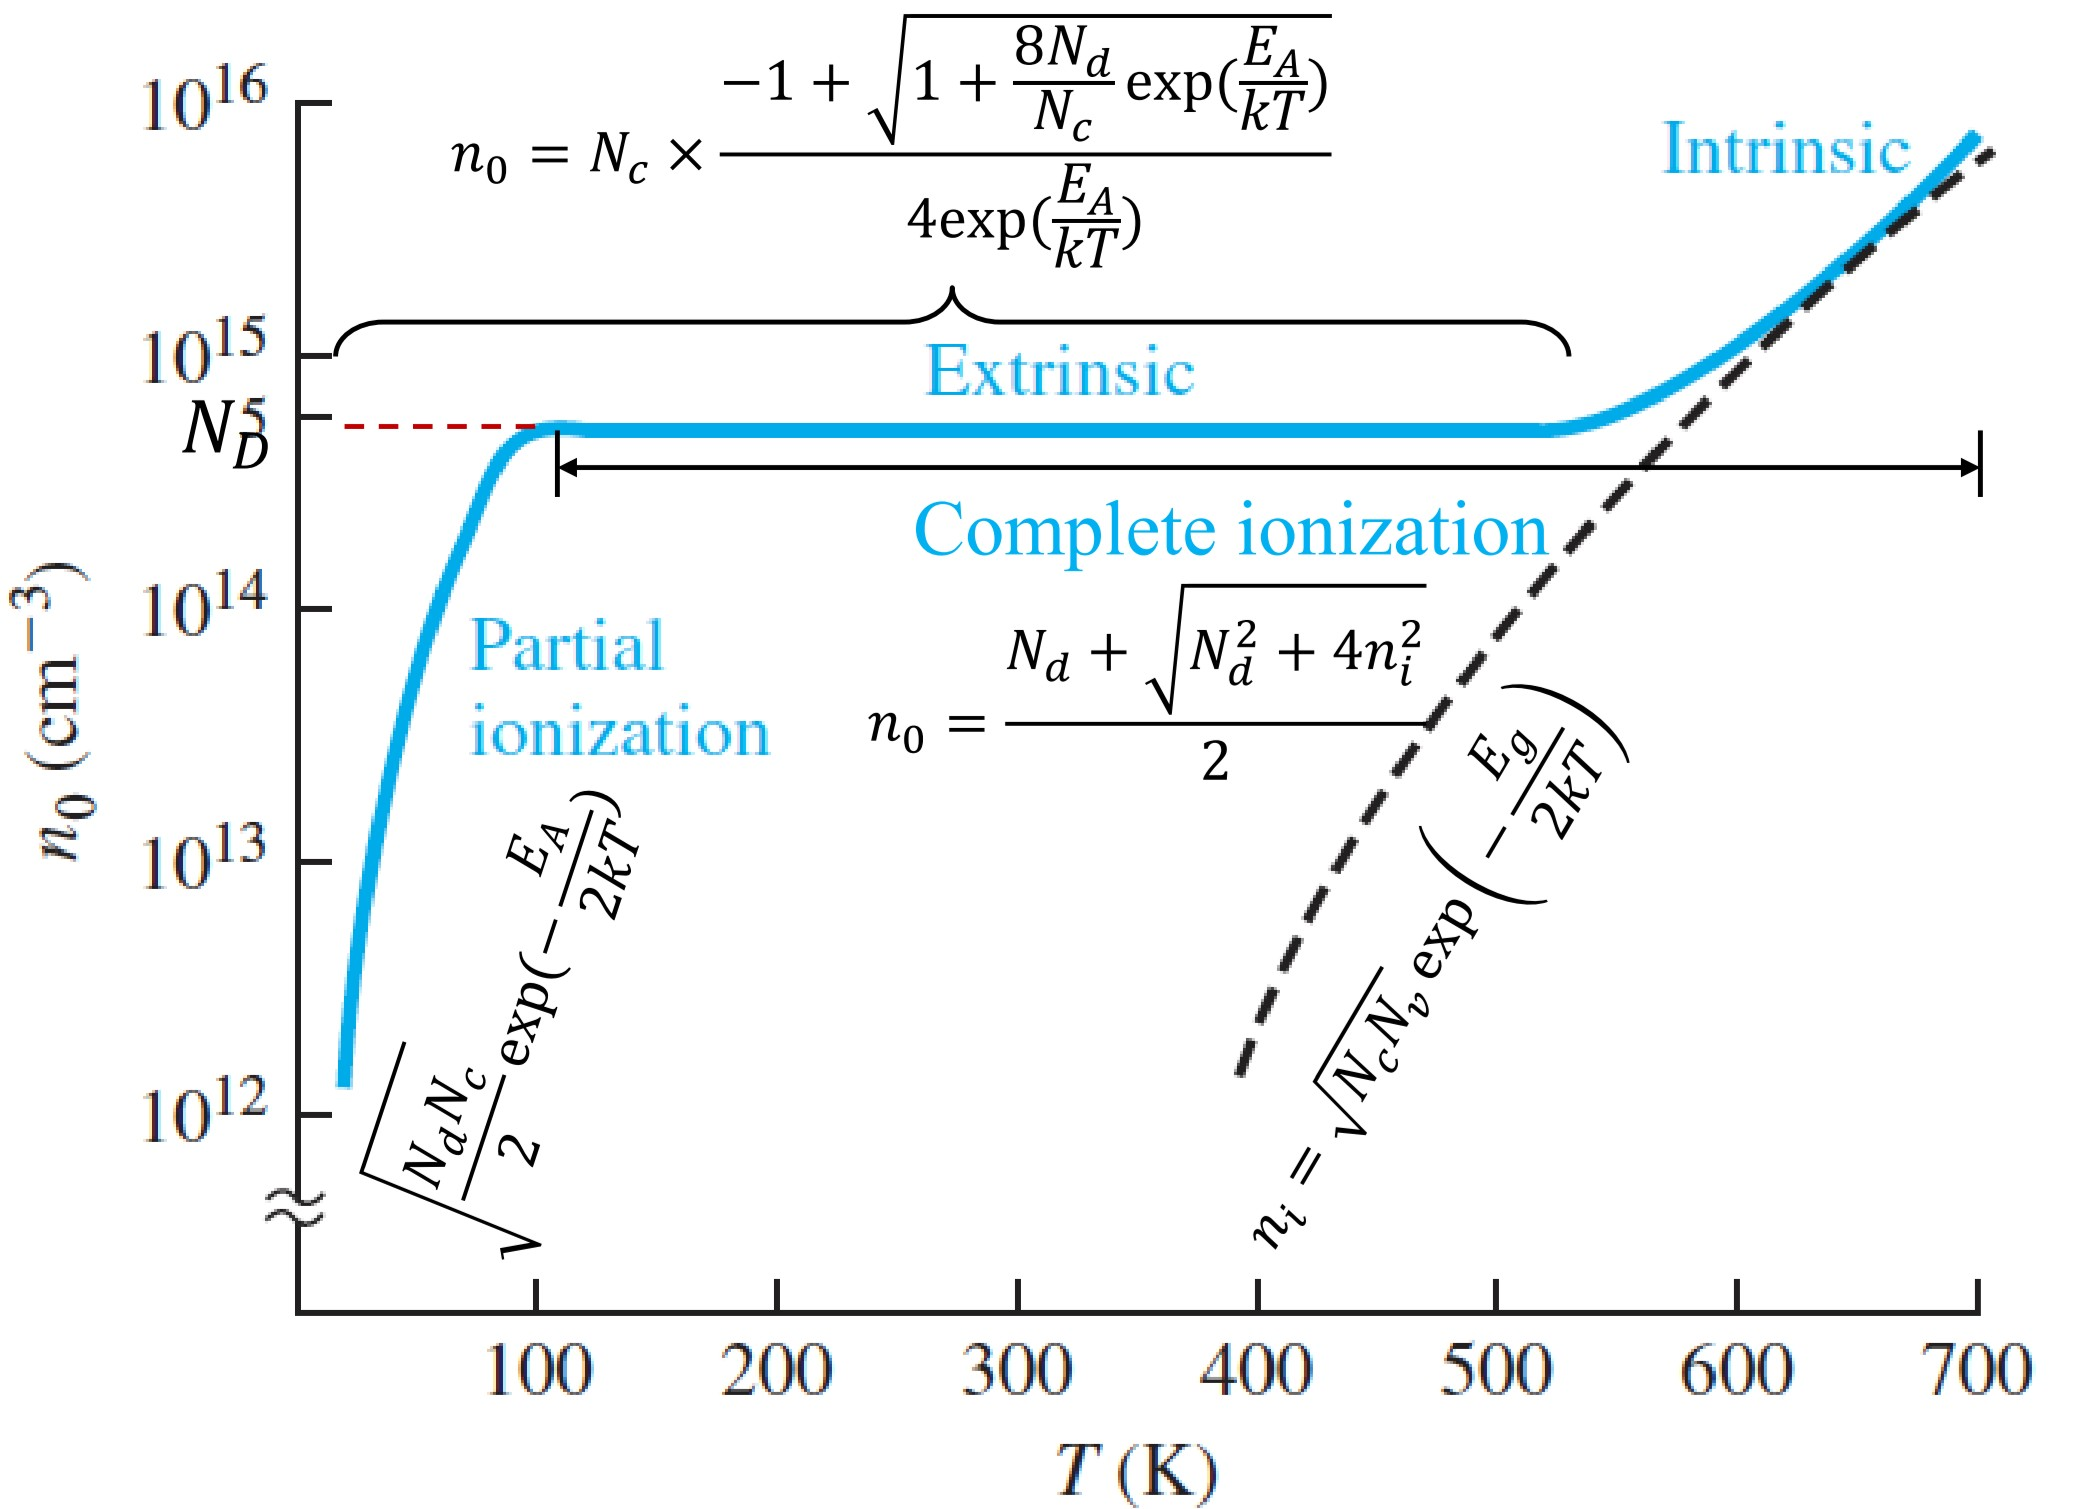
\includegraphics[width=0.6\linewidth]{Ionization-of-dopants.jpg}
                    \label{fig:Ionization-of-dopants.jpg}
                \end{figure}
                \begin{equation*}
                    n_0 = \int_{E_c}^\infty g_c(E) f_F(E) \d E = N_c \exp\left( \frac{E_F - E_c}{kT}  \right)
                \end{equation*}
        \end{itemize}
    \end{frame}

    \begin{frame} \frametitle{Overview}
        \begin{itemize}
            \item \textbf{Chapter 3} Introduction to the Quantum Theory of Solids
                \begin{equation*}
                    \begin{aligned}
                        g(E) &= \frac{4 \pi (2m)^{\frac{3}{2} }}{h^3} \sqrt{E}  \\
                        f_F(E) &= \frac{1}{1 + \exp\left( \frac{E - E_F}{kT}  \right)} \\
                    \end{aligned}
                \end{equation*}
                \begin{figure}[H]
                    \centering
                    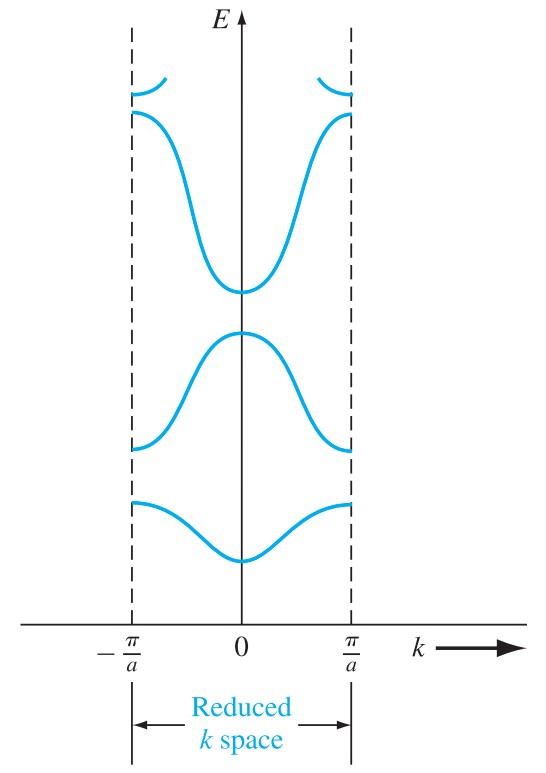
\includegraphics[height=7em]{E-k-diagram.jpg}
                    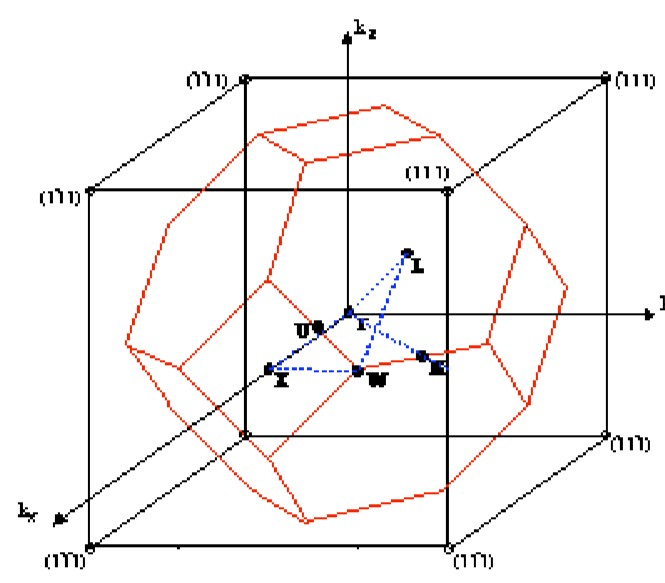
\includegraphics[height=7em]{3D-structure.jpg}
                    \label{fig:E-k-diagram.jpg}
                \end{figure}
        \end{itemize}
    \end{frame}

    \begin{frame} \frametitle{Overview}
        \begin{itemize}
            \item \textbf{Chapter 2} Quantum Mechanics
                \begin{equation*}
                    E = \frac{k^2 \hbar^2}{2m} 
                \end{equation*}

            \item \textbf{Chapter 1} Introduction
        \end{itemize}
    \end{frame}



\section{Chapter 1 The Crystal Structure of Solids}
    \begin{frame} \frametitle{Lattice types}
        \begin{figure}[H]
            \centering
            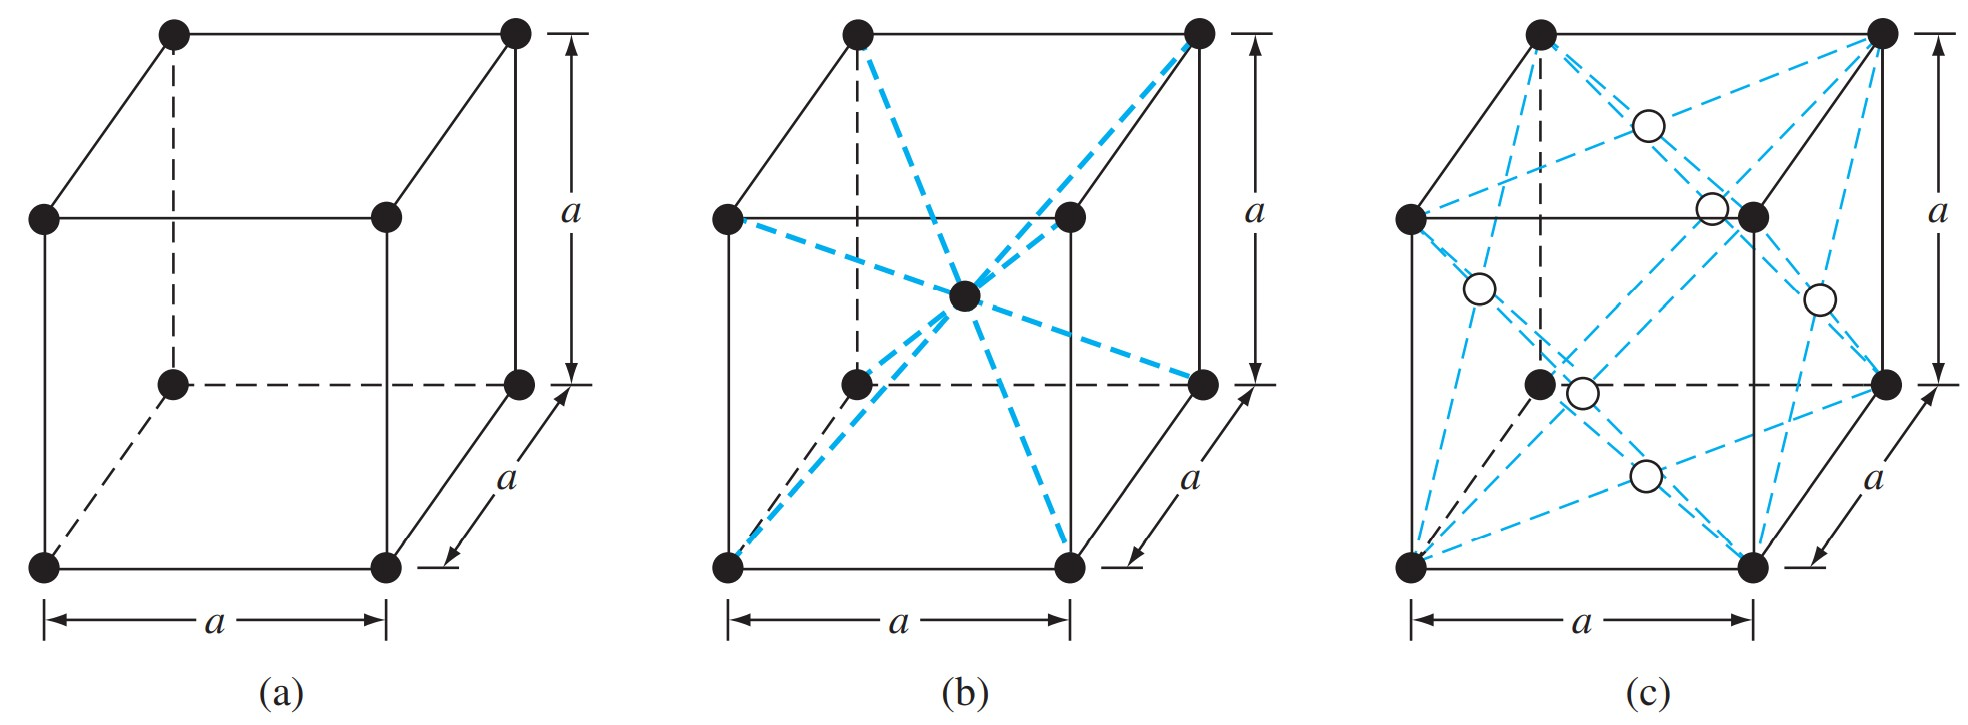
\includegraphics[width=0.9\linewidth]{Lattice_types.jpg}
            \caption{\tiny (a) simple cubic(\textcolor{red}{sc}), (b) body-centered cubic(\textcolor{red}{bcc}), (c) face-centered cubic(\textcolor{red}{fcc})}
            \label{fig:Lattice_types.jpg}
        \end{figure}
        \begin{equation*}
            \# \text{number of atoms per unit cell}
        \end{equation*}
        % volume density of atoms
        \begin{equation*}
            \text{Volume Density} = \frac{\text{\# atoms per unit cell}}{\text{volume of unit cell}} 
        \end{equation*}
        % Surface density of atoms
        \begin{equation*}
            \text{Surface Density} = \frac{\text{\# atoms per lattice plane}}{\text{area of lattice plane}}
        \end{equation*}
    \end{frame}
    

    \begin{frame} \frametitle{The diamond structure}
        \par \textbf{The diamond structure } all atoms are of the same species
        \par \textbf{The zincblende structure } two different types of atoms. e.g, GaAs.
        % TODO: check this
        % No two atoms of same type are connected together.
        \begin{figure}[H]
            \centering
            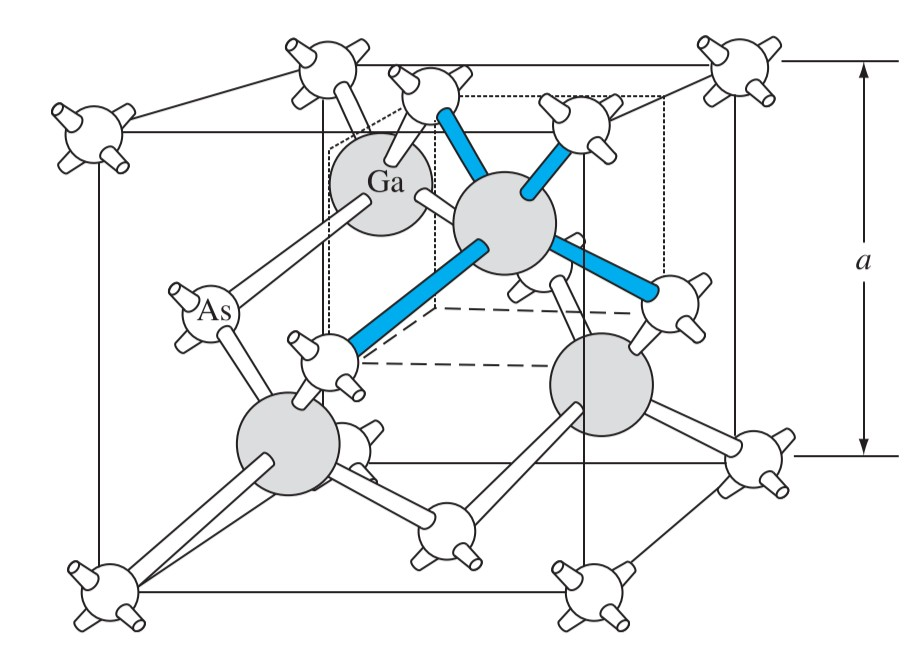
\includegraphics[width=0.5\linewidth]{GaAs_zincblende.jpg}
            \label{fig:GaAs_zincblende.jpg}
        \end{figure}
        \par Equivalent to two face-centered cubics sliding $1/4$ diagonal length along a diagonal.


        \begin{center}
            \# atoms per unit cell $= 8$.
        \end{center}
    \end{frame}


    \begin{frame} \frametitle{Crystalline Plane and Miller Index}
        \begin{figure}[H]
            \centering
            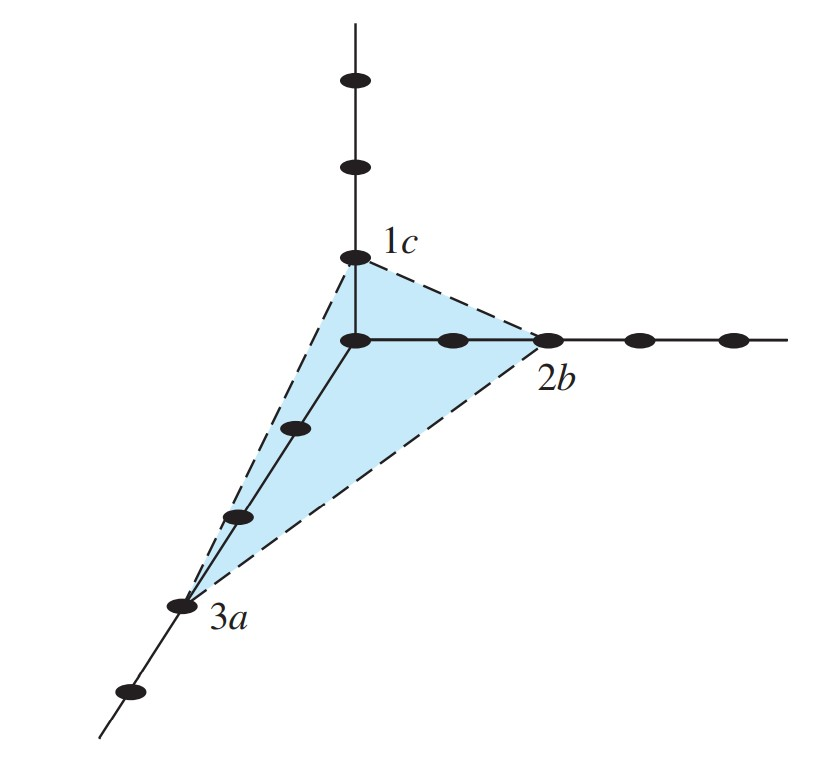
\includegraphics[width=0.4\linewidth]{Miller-index-1.jpg}
            \label{fig:Miller-index-1.jpg}
        \end{figure}
        % \par Intercepts: $(3,2,1)$.
        % \par Reciprocal: $(\frac{1}{3}, \frac{1}{2} , 1 )$.
        % \par Multiplying the lowest common denominator (lcd): $(2,3,6)$.
        \begin{equation*}
            (3,2,1) \stackrel{\text{Reciprocal}}{\longrightarrow} (\frac{1}{3} , \frac{1}{2} , 1) \stackrel{\text{multiply lcd}}{\longrightarrow} (2,3,6)
        \end{equation*}
        \par Any parallel plane is entirely equivalent to any other.
        \par The $[hkl]$ \underline{direction} is perpendicular to the $(hkl)$ \underline{plane}. \\[1em]
        \par \textbf{\textcolor{blue}{Example}}: Determine the Miller index of x-y plane.
    \end{frame}


\section{Chapter 2 Introduction to Quantum Mechanics}
    \begin{frame} \frametitle{Infinite quantum well}
        \begin{equation*}
            - \frac{\hbar^2}{2m} \frac{\partial^2 \Psi}{\partial x^2} + V(x) \Psi = E \Psi  , \quad \left\{
                \begin{array}{ll}
                    V(x) = + \infty, & x \le 0 \text{ or } x \ge a \\
                    V(x) = 0, & 0 < x < a
                \end{array}
            \right.
        \end{equation*}
        General solution:
        \begin{equation*}
            \Psi (x) = A \e^{-ikx} + B \e^{ikx} 
        \end{equation*}
        Boundary condition:
        \begin{equation*}
            \begin{aligned}
            % \left\{
                % \begin{array}{ll}
                    & \Psi (x) | _{x = a, 0} = 0 \\
                    & \int_{0}^{a} \Psi(x) \Psi^*(x) \d x = 1 \\
                % \end{array}
            % \right.
            \end{aligned}
        \end{equation*}
        conclusion:
        \begin{equation*}
            \begin{aligned}
                &k = \frac{n\pi}{a} , n = 0, \pm 1, \pm 2, \dots \\
                &E = \frac{k^2 \hbar^2}{2m} = \frac{n^2 \pi^2 \hbar^2}{2m a^2}  
            \end{aligned}
        \end{equation*}
    \end{frame}


    \begin{frame} \frametitle{Finite quantum well}
        \begin{equation*}
            - \frac{\hbar^2}{2m} \frac{\partial^2 \Psi}{\partial x^2} + V(x) \Psi = E \Psi  , \quad \left\{
                \begin{array}{ll}
                    V(x) = V_0, & x \le 0 \text{ or } x \ge a \\
                    V(x) = 0, & 0 < x < a
                \end{array}
            \right.
        \end{equation*}
        General solution:
        \begin{equation*}
            \Psi(x) = 
            \left\{
                \begin{array}{lll}
                    A \e^{-i k_1 x} + B \e^{ik_1 x}, & k_1 = \sqrt{\frac{2m(E - V_0)}{\hbar^2} } , & x \le 0\text{ or }x \ge a \\
                    C \e^{-ik_2x} + D \e^{ik_2 x}, & k_2 = \sqrt{\frac{2mE}{\hbar^2} } , & 0 < x < a 
                \end{array}
            \right.
        \end{equation*}
        Boundary condition:
        \begin{equation*}
            \begin{aligned}
            % \left\{
                % \begin{array}{ll}
                    & \Psi (x) | _{x = 0} \text{ continuous}\\
                    & \Psi (x) | _{x = a} \text{ continuous}\\
                    & \int_{-\infty}^{\infty} \Psi(x) \Psi^*(x) \d x = 1 \\
                % \end{array}
            % \right.
            \end{aligned}
        \end{equation*}
        Note: depending on the relationship between $E$ and $V_0$, $\Psi(x)$ is different.
    \end{frame}


    \begin{frame} \frametitle{Energy bands}
        \begin{figure}[H]
            \centering
            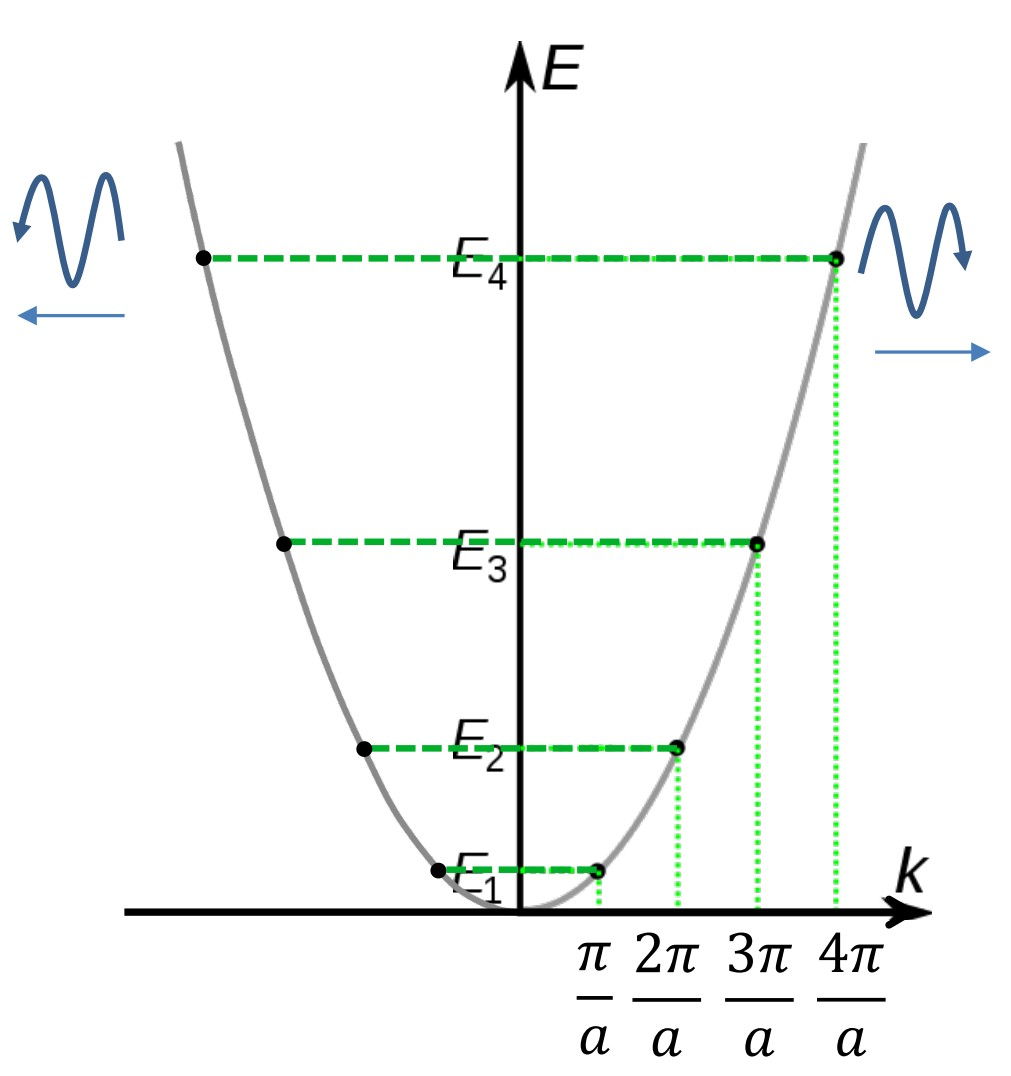
\includegraphics[width=0.3\linewidth]{Energy-level.jpg}
            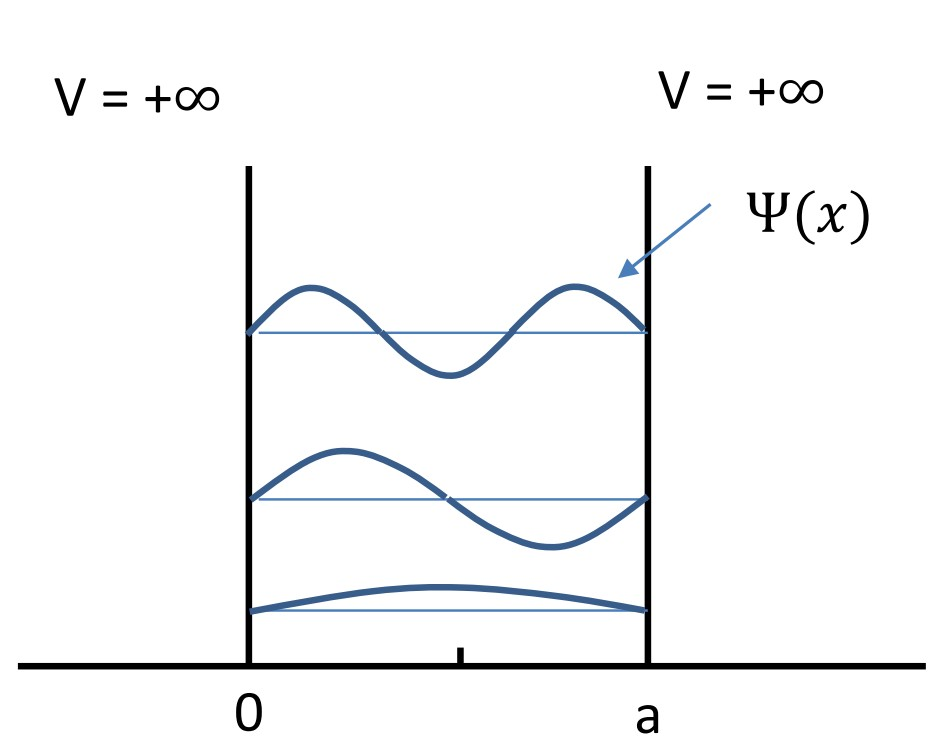
\includegraphics[width=0.3\linewidth]{Wave-function-infinite.jpg}
            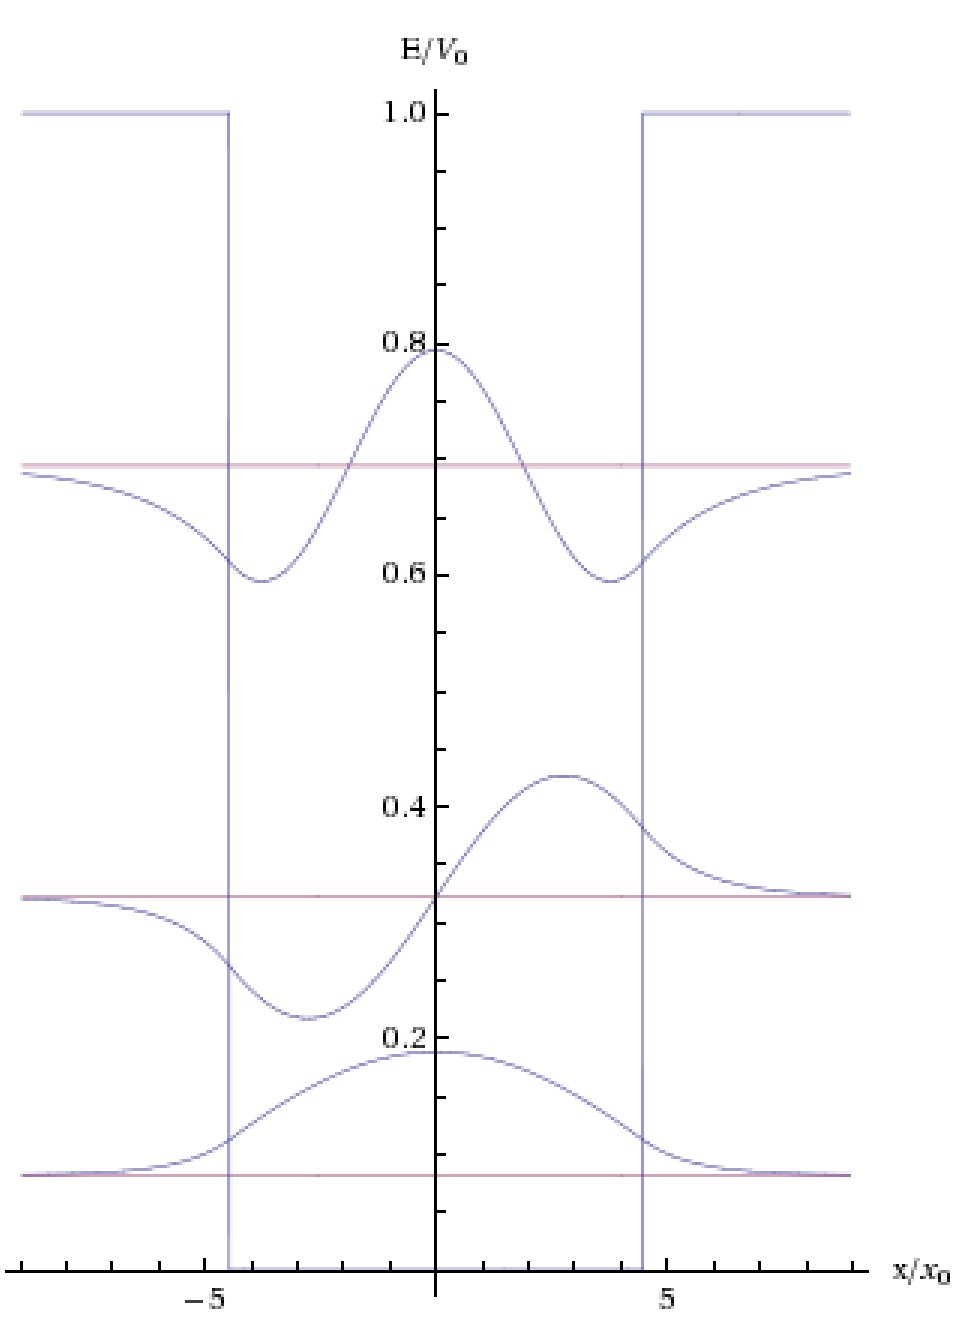
\includegraphics[width=0.3\linewidth]{Wave-function-finite.jpg}
            \label{fig:Energy_bands.jpg}
        \end{figure}
        \par For same energy level, the $k$ can have two values, Because the wave can move to positive and negative directions.
    \end{frame}



\section{Chapter 3 Introduction to the Quantum Theory of Solids}
    \begin{frame} \frametitle{Effective mass}
        \begin{figure}[H]
            \vspace{-0.5em}
            \centering
            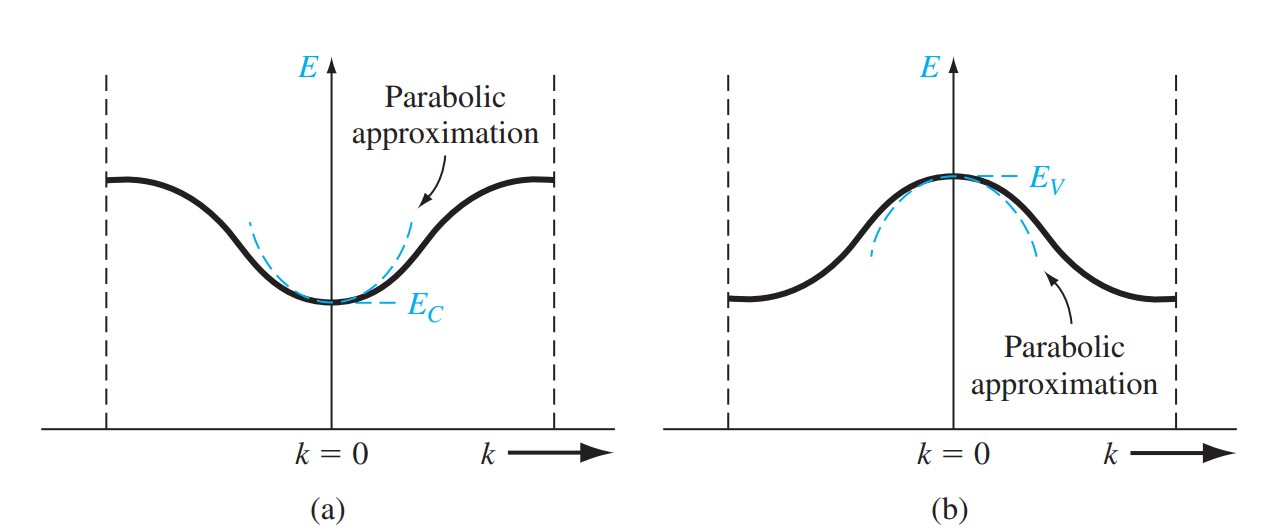
\includegraphics[width=0.8\linewidth]{Effective-mass.jpg}
            % \caption{\tiny (a) The conduction band in reduced k space, and the parabolic approximation. (b) The valence band in reduced k space, and the parabolic approximation}
            \label{fig:Effective-mass.jpg}
            \vspace{-0.5em}
        \end{figure}

        \begin{equation*}
            \boxed{\frac{1}{\hbar^2} \frac{\d^2 E}{\d k^2} = \frac{2C_1}{\hbar^2} = \frac{1}{m^*}  }
        \end{equation*}
        \begin{equation*}
            \begin{aligned}
                E = E(k) = E_c + \frac{\hbar^2}{2m_n^*} (k - k_1)^2 \\
                E = E(k) = E_v - \frac{\hbar^2}{2m_p^*} (k - k_2)^2
            \end{aligned}
        \end{equation*}
    \end{frame}

    \begin{frame} \frametitle{Effective Mass: experimentally}
        Cyclotron resonance
        \begin{figure}[H]
            \centering
            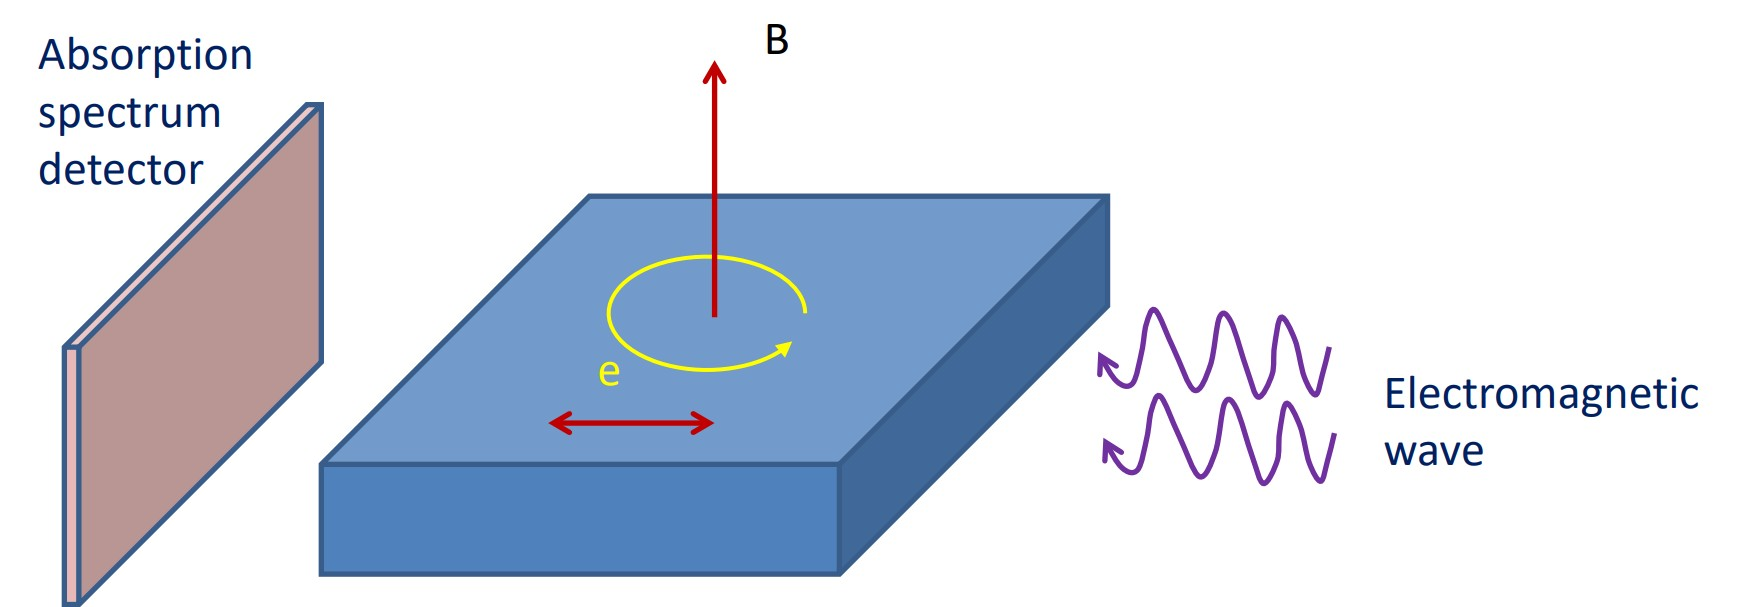
\includegraphics[width=0.6\linewidth]{Effective-mass-experiment.jpg}
            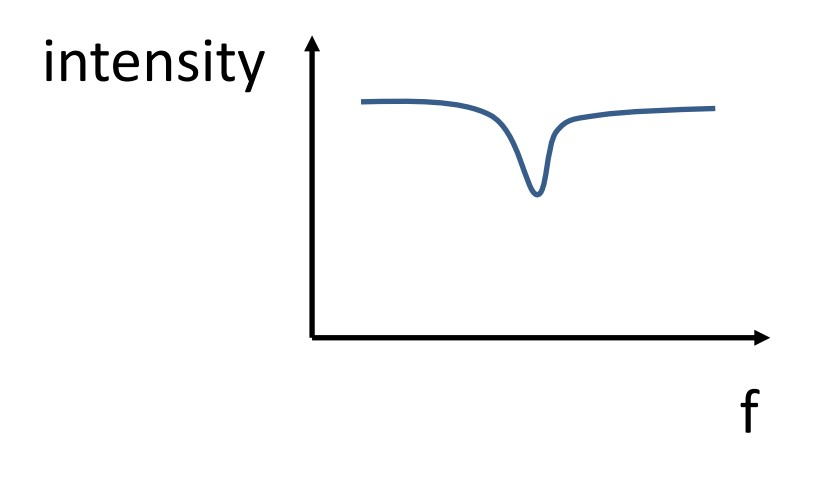
\includegraphics[width=0.3\linewidth]{Effective-mass-experiment-graph.jpg}
            \label{fig:Effective-mass-experiment.jpg}
        \end{figure}
        \begin{equation*}
            \boxed{m^* = \frac{eB\lambda}{2\pi c} }
        \end{equation*}
    \end{frame}

    \begin{frame} \frametitle{Density of States Function}
        \begin{figure}[H]
            \centering
            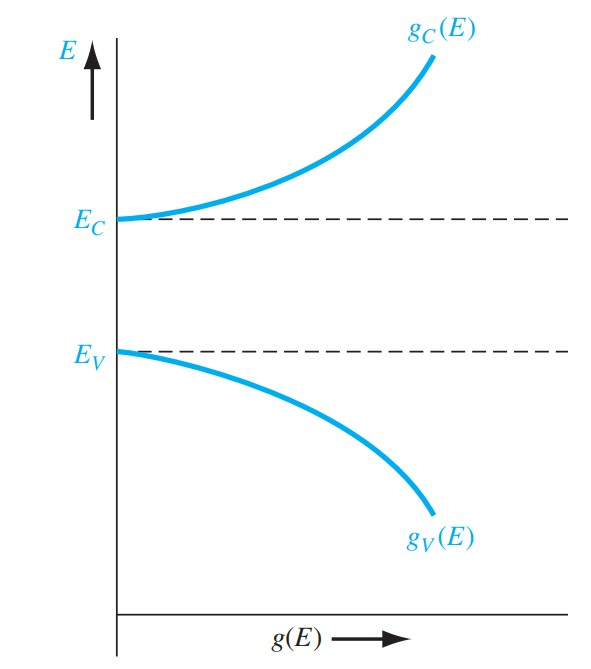
\includegraphics[width=0.3\linewidth]{Density-state-function.jpg}
            \label{fig:Density-state-function.jpg}
        \end{figure}
        \begin{equation*}
            \boxed{
                \begin{aligned}
                    g(E) &= \frac{4 \pi (2m)^{\frac{3}{2} }}{h^3} \sqrt{E}  \\
                    g_c(E) &= \frac{4 \pi (2m_n^*)^{\frac{3}{2} }}{h^3} \sqrt{E - E_c}  \\
                    g_v(E) &= \frac{4 \pi (2m_p^*)^{\frac{3}{2} }}{h^3} \sqrt{E_v - E}  \\
                \end{aligned}
            }
        \end{equation*}
    \end{frame}

    \begin{frame} \frametitle{Distribution Function}
        \begin{itemize}
            \item Fermi-Dirac probability function:
                \begin{equation*}
                    f_F(E) = \frac{1}{1 + \exp\left( \frac{E - E_F}{kT}  \right)} 
                \end{equation*}
                \begin{figure}[H]
                    \centering
                    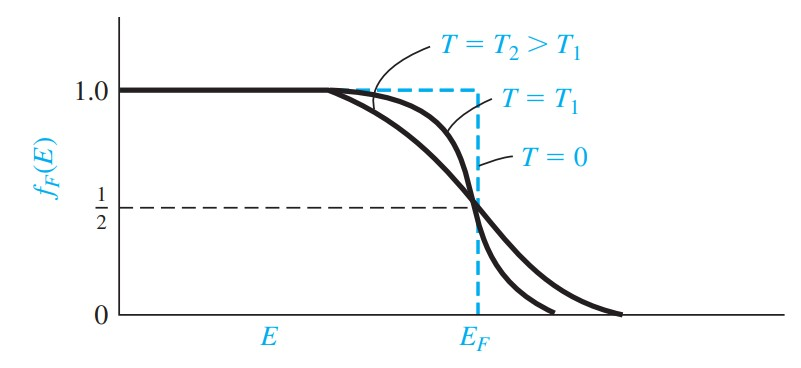
\includegraphics[width=0.8\linewidth]{Fermi-distribution.jpg}
                    \label{fig:Fermi-distribution.jpg}
                \end{figure}
        \end{itemize}
    \end{frame}

    \begin{frame} \frametitle{Distribution Function}
        \begin{itemize}
            \item Boltzmann distribution
                \par When $\exp \left( \frac{E - E_F}{kT} \right) >> 1 \Rightarrow E - E_F > 3kT$
                \begin{equation*}
                    f_F(E) \approx exp\left( -\frac{E - E_F}{kT}  \right)
                \end{equation*}
                \begin{figure}[H]
                    \centering
                    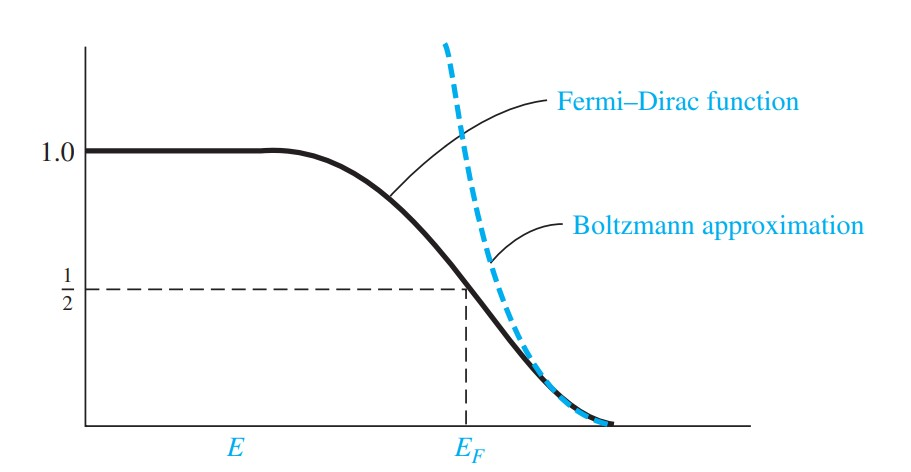
\includegraphics[width=0.8\linewidth]{Boltzmann-distribution.jpg}
                    \label{fig:Boltzmann-distribution.jpg}
                \end{figure}
        \end{itemize}
    \end{frame}


\section{Chapter 4 The semiconductor in Equilibrium}
    \begin{frame} \frametitle{$n_0$ and $p_0$ Equations}
        \begin{equation*}
            \begin{aligned}
                &n_0 = \int_{E_c}^\infty g_c(E) f_F(E) \d E \\
                \Rightarrow \quad &\boxed{n_0 = N_c \exp \left[ \frac{-(E_c - E_F)}{kT}  \right], \quad N_c = 2 \left( \frac{2\pi m_n^* kT}{h^2}  \right)^{3/2}} \\
                &p_0 = \int_{-\infty}^{E_v} g_v(E) \left(1 - f_F(E)\right) \d E \\
                \Rightarrow \quad &\boxed{p_0 = N_v \exp\left[ \frac{-(E_F - E_v)}{kT}  \right], \quad N_v = 2 \left( \frac{2\pi m_p^* kT}{h^2}  \right)^{3/2}}
            \end{aligned}
        \end{equation*}

        \begin{center}
            \underline{$kT = 0.0259$ only for $T = 300K$}
        \end{center}
        \begin{center}
            \textcolor{red}{Always be careful about the temperature!} 
        \end{center}
    \end{frame}

    \begin{frame} \frametitle{Intrinsic Semiconductor}
        \begin{equation*}
            \boxed{n_0 p_0 = n_i^2 = N_cN_v \exp \left[ \frac{-(E_c - E_v)}{kT}  \right] = N_c N_v \exp \left[ \frac{-E_g}{kT}  \right]}
        \end{equation*}
        \begin{equation*}
            \boxed{E_{Fi} - E_{midgap} = \frac{1}{2} kT \ln \left( \frac{N_v}{N_c}  \right) = \frac{3}{4} kT \ln \left( \frac{m_p^*}{m_n^*}  \right)}
        \end{equation*}
    \end{frame}

    \begin{frame}[t] \frametitle{Self-consistency}
        \begin{equation*}
            n_i^2 = N_cN_v \exp \left[ \frac{-(E_c - E_v)}{kT}  \right] = N_c N_v \exp \left[ \frac{-E_g}{kT}  \right]
        \end{equation*}
        \vspace{2em}
        \par For $Si$ at $300K$:
        \begin{equation*}
            \begin{aligned}
                &n_i = 1.5 \times 10^{10} cm^{-3},\\ &E_g = 1.12 eV, \\ 
                &N_c = 2.8 \times 10^{19} cm^{-3},\\ &N_v = 1.04 \times 10^{19} cm^{-3},\\ &kT = 0.0259 eV
            \end{aligned}
        \end{equation*}
        \begin{equation*}
            LHS = 2.25 \times 10^{20} {\color{red} \neq } 4.82936 \times 10^{19} = RHS  
        \end{equation*}

        \begin{center}
            \textcolor{red}{Write down the steps with all equations and constants used!} 
        \end{center}
    \end{frame}

    \begin{frame} \frametitle{The Extrinsic Semiconductor}
        \begin{figure}[H]
            \centering
            \begin{subfigure}[b]{0.45\linewidth}
                \centering
                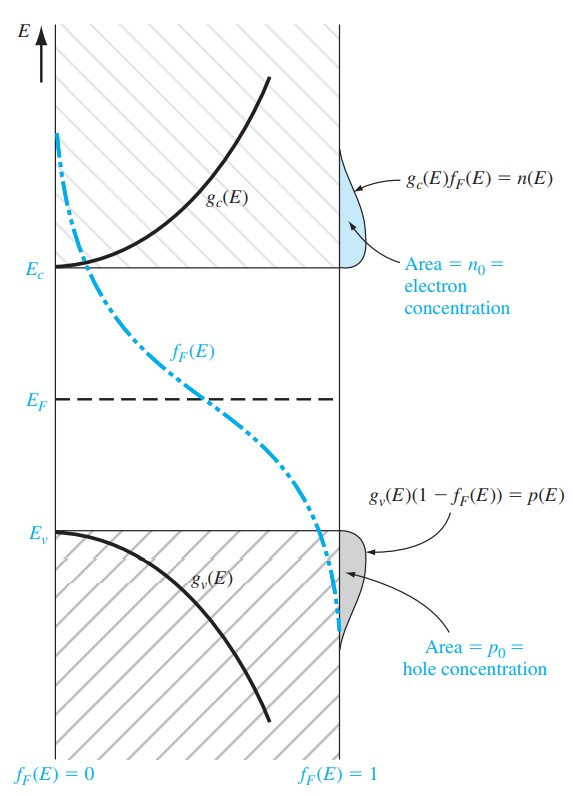
\includegraphics[height=4cm]{Intrinsic.jpg}
                \caption{Intrinsic}
                \label{subfig:Intrinsic.jpg}
            \end{subfigure}
            \begin{subfigure}[b]{0.45\linewidth}
                \centering
                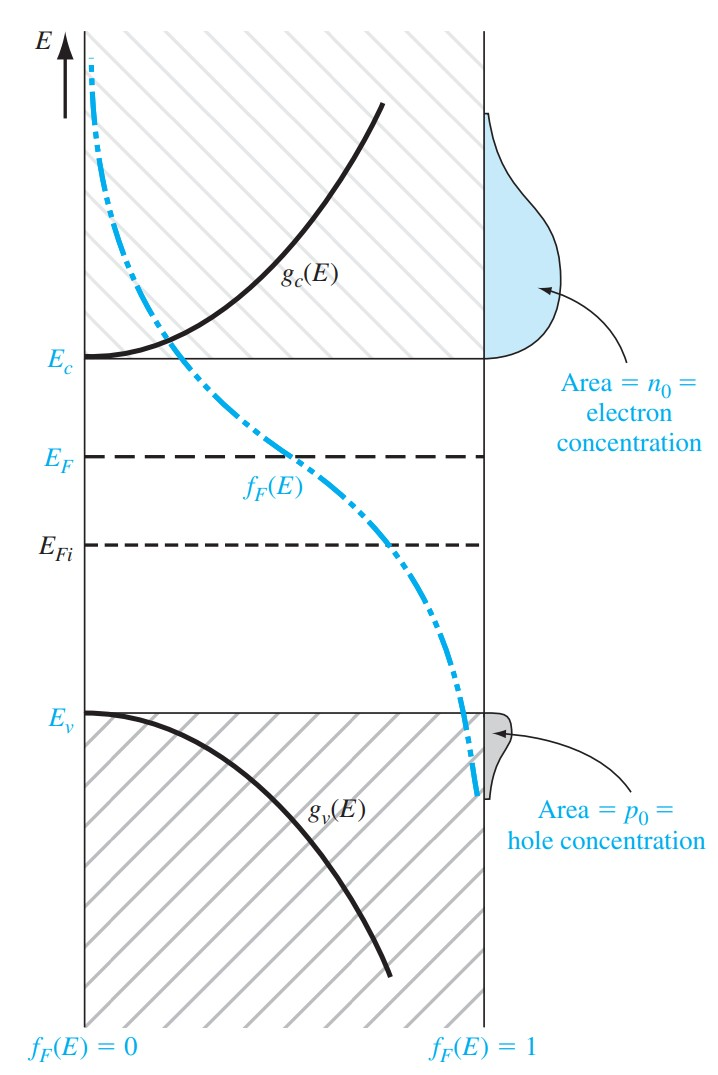
\includegraphics[height=4cm]{Extrinsic-n-type.jpg}
                \caption{n-type semiconductor}
                \label{subfig:Extrinsic-n-type.jpg}
            \end{subfigure}
            % \caption{Density of states functions, Fermi-Dirac probability function, and areas representing electron and hole concentrations}
            \label{fig:subcaption-of-dopants}
        \end{figure}
        \begin{equation*}
            \boxed{n_0p_0 = N_c N_v \exp \left( -\frac{E_g}{kT}  \right) = n_i^2}
        \end{equation*}
    \end{frame}

    \begin{frame} \frametitle{Statistics of Donors and Acceptors}
        \begin{figure}[H]
            \centering
            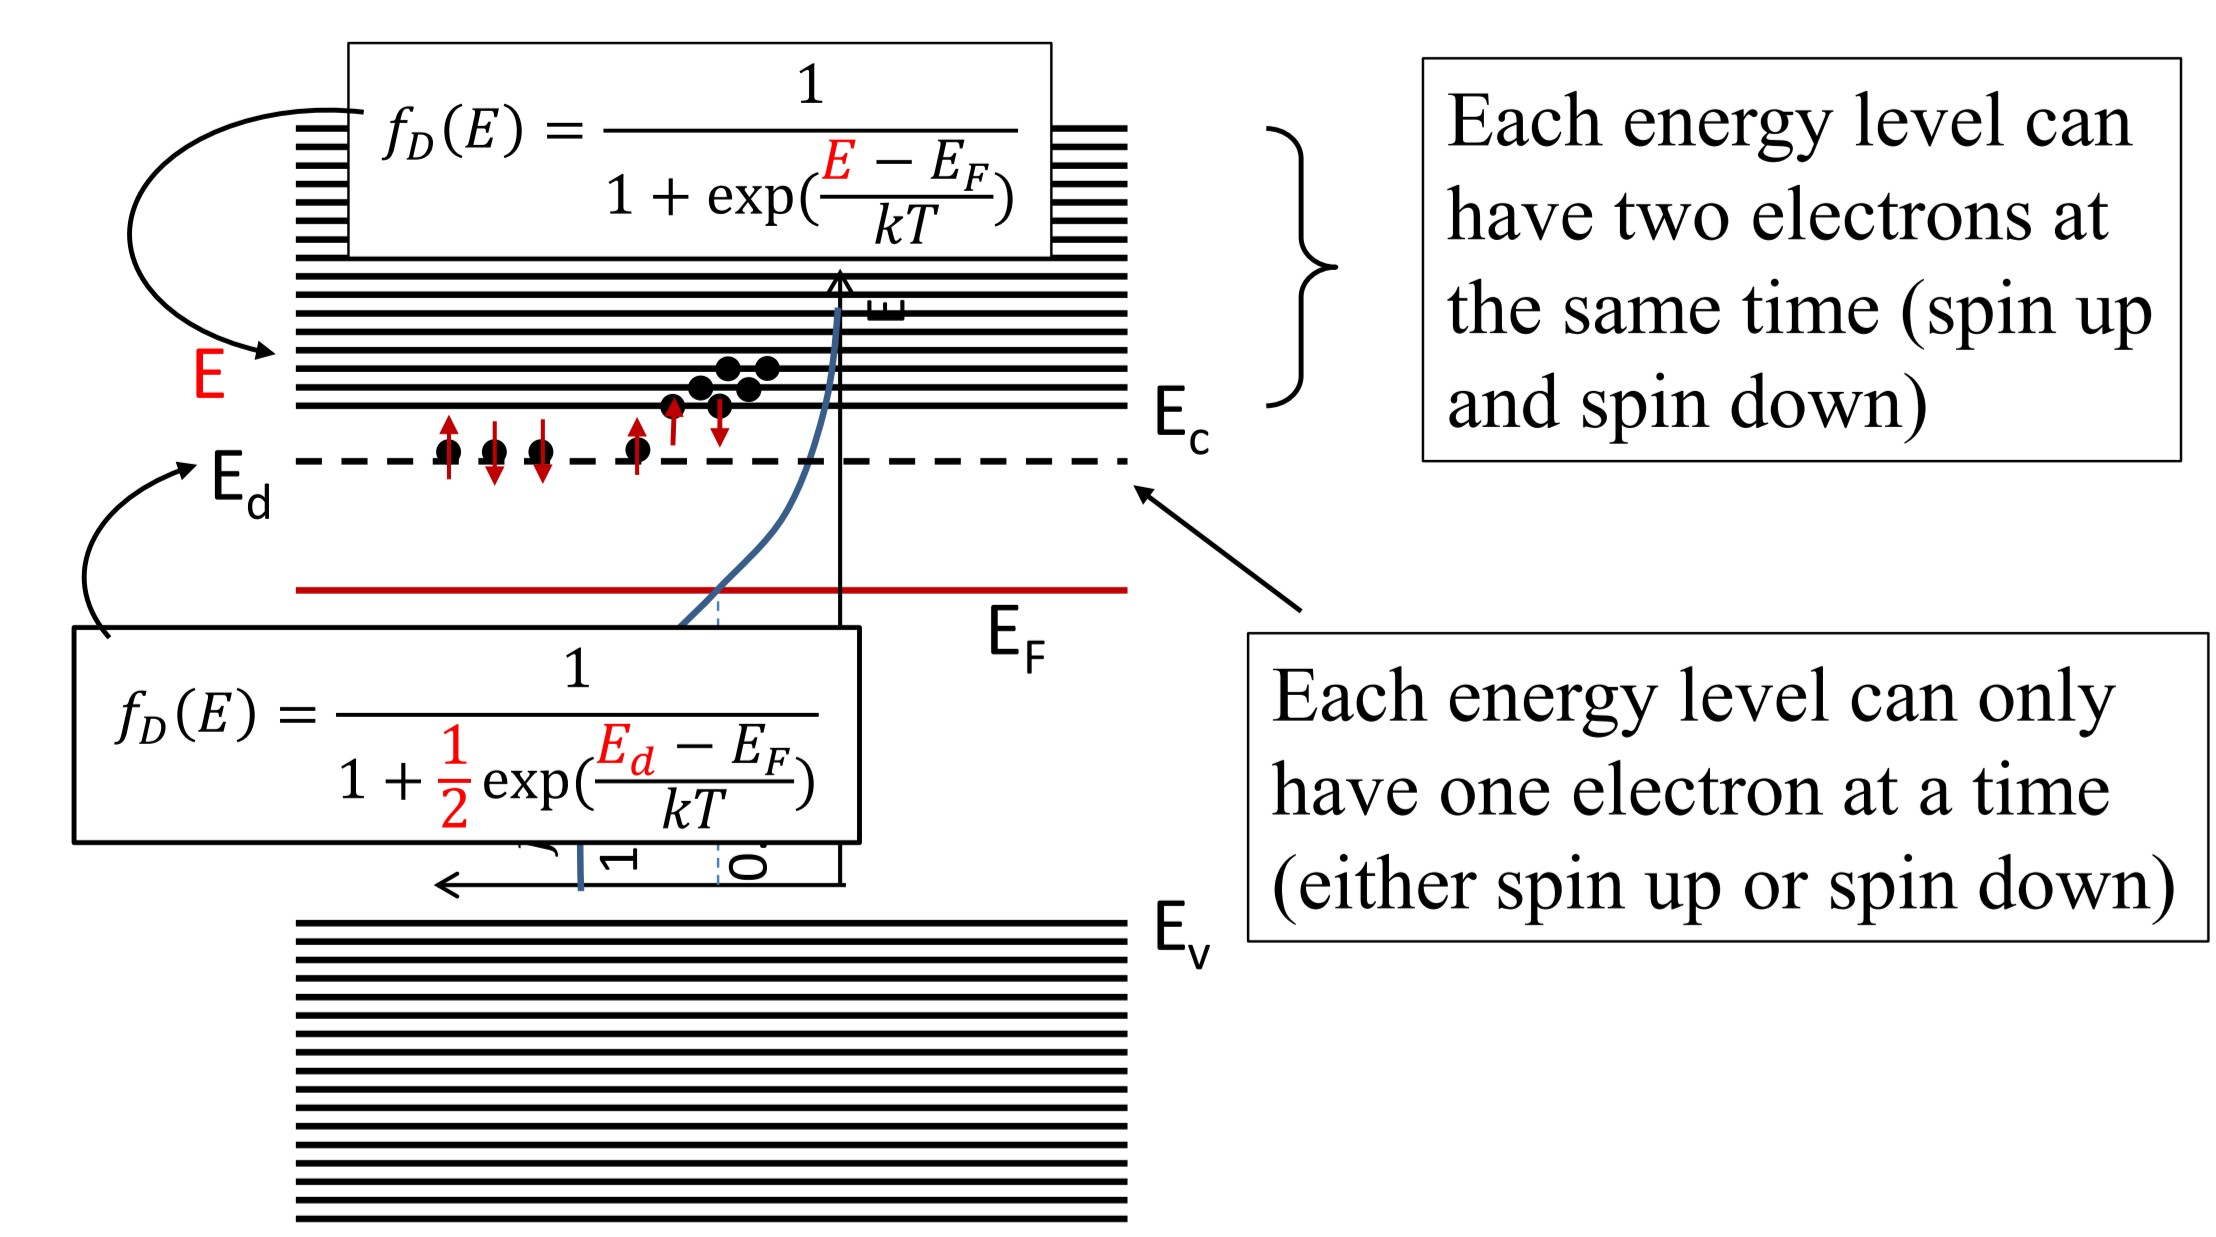
\includegraphics[width=0.9\linewidth]{Probability-function-donors.jpg}
            \label{fig:Probability-function-donors.jpg}
        \end{figure}
    \end{frame}

    \begin{frame} \frametitle{Statistics of Donors and Acceptors}
        \begin{equation*}
            f_d(E) = \frac{1}{1 + \frac{1}{2} \exp \left( \frac{E_d - E_F}{kT}  \right)} 
        \end{equation*}
        \begin{equation*}
            n_d = f_d(E) N_d = N_d - N_d^+
        \end{equation*}
        where $N_d^+$ is the concentration of ionized donors.

        \begin{equation*}
            f_a(E) = \frac{1}{1 + \frac{1}{g} \exp\left( \frac{E_F - E_a}{kT}  \right)} 
        \end{equation*}
        $1/g$ is the degeneracy factor, normally taken as $4$ for acceptor level in silicon and gallium arsenide (because of detailed band structure). 
        \begin{equation*}
            p_a = f_a(E) N_a = N_a - N_a^+
        \end{equation*}
    \end{frame}

    \begin{frame} \frametitle{Statistics of Donors and Acceptors}
        
        \par We calculate the relative number of electrons in the donor state compared with the total number of electrons: (assuming $(E_d - E_F) \gg  kT$)
        \begin{equation*}
            \frac{n_d}{n_d + n_0} = \frac{1}{1 + \frac{N_c}{2N_d} \exp\left[ \frac{-(E_c - E_d)}{kT}  \right]} 
        \end{equation*}
        \par \textbf{\textcolor{blue}{Example}:} Determine the fraction of total electrons still in the donor states at $T = 300 K$. Consider phosphorus doping in silicon, for $T = 300 K$, at a concentration of $N_d = 10^{16} cm^{-3}$.
        \par \textbf{\textcolor{blue}{Answer}:} $0.41\%$. Very few electrons remains in the donor states (completely ionized).
    \end{frame}

    \begin{frame} \frametitle{}
        \begin{figure}[H]
            \centering
            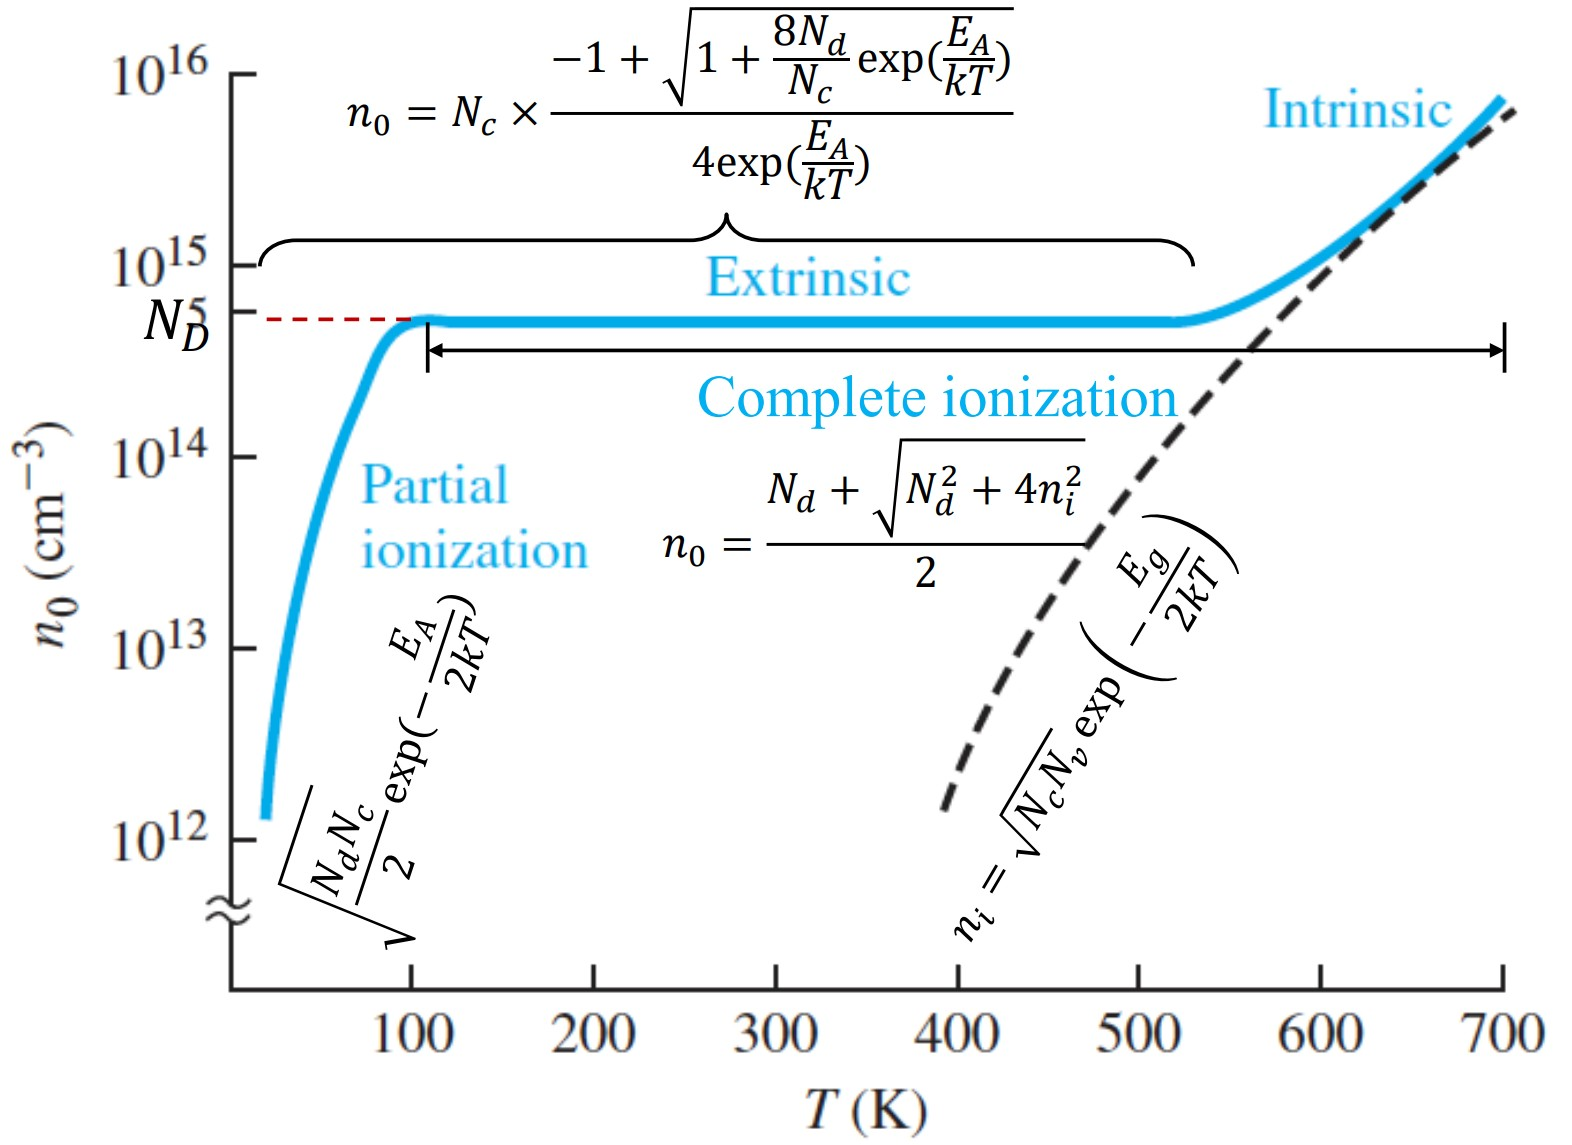
\includegraphics[width=0.95\linewidth]{n0-versus-T.jpg}
            \label{fig:n0-versus-T-0.jpg}
        \end{figure}
    \end{frame}

    \begin{frame} \frametitle{Fermi Level Position}
        \begin{equation*}
            \begin{aligned}
                E_F &= E_c + kT \ln \left( \frac{\sqrt{1 + \frac{8 N_d}{N_c} \exp\left( \frac{E_A}{kT}  \right)} - 1}{4 \exp\left( \frac{E_A}{kT}  \right)}  \right) \\
                &= \left\{
                    \begin{aligned}
                        \frac{E_c + E_D}{2} +\frac{kT}{2} \ln \frac{N_d}{2N_c}, &\quad  T \text{ small} \\
                        E_c - kT \ln \frac{N_c}{N_d}, &\quad  T \text{ big}
                    \end{aligned}
                \right.
            \end{aligned}
        \end{equation*}
        \begin{figure}[H]
            \centering
            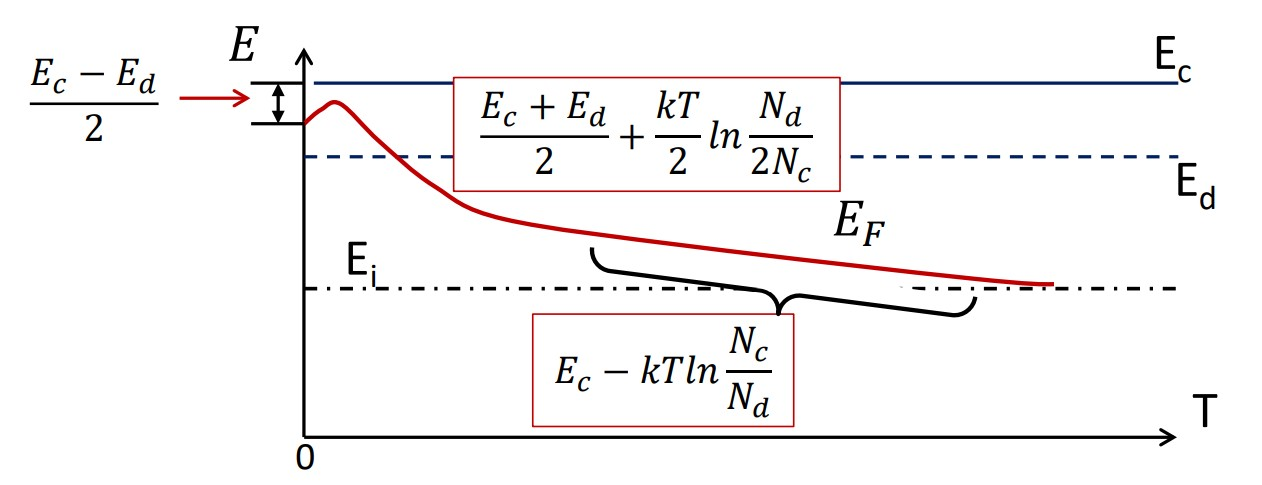
\includegraphics[width=0.8\linewidth]{Fermi-level-position.jpg}
            \label{fig:Fermi-level-position.jpg}
        \end{figure}
    \end{frame}


    % \begin{frame} \frametitle{}
    %     \begin{equation*}
    %         \begin{aligned}
    %             E_x &= - \frac{\d \Phi}{\d x} = \frac{1}{e} \frac{\d E_{Fi}}{\d x} \\
    %             &= - \frac{1}{e} \frac{kT}{n(x)} \frac{\d n(x)}{\d x} 
    %         \end{aligned}
    %     \end{equation*}
    % \end{frame}



    \begin{frame} 
        \begin{center}
            \Large\textcolor{blue}{Good luck to your midterm exam!} \\
            \textcolor{white}{Golden egg} 
        \end{center}
    \end{frame}

\end{document} 